% Basic settings
\documentclass[a4paper,10pt]{article}
\usepackage[utf8]{inputenc}
\usepackage[german]{babel}

% Layout settings
\usepackage[top=1.5cm, bottom=1.5cm, left=1.5cm, right=1.5cm]{geometry}
\usepackage[compact]{titlesec}
\titlespacing{\section}{0pt}{0pt}{0pt}
\titlespacing{\subsection}{0pt}{0pt}{0pt}
\titlespacing{\subsubsection}{0pt}{0pt}{0pt}
\setlength{\parindent}{0em}
\setlength{\parskip}{1em}

% Two columns
\usepackage{multicol}

% Colored boxes
\usepackage[most]{tcolorbox}

% package to get colored text
\usepackage{xcolor}

% A base set of colorbox that is then customised
\tcbset {
    base/.style={
        boxrule=0mm,
        leftrule=1mm,
        left=1.75mm,
        arc=0mm,
        fonttitle=\bfseries,
        colbacktitle=black!10!white,
        coltitle=black,
        toptitle=0.75mm,
        bottomtitle=0.25mm,
        title={#1}
    }
}

% Box with red line for definitions
\definecolor{bittersweet}{rgb}{1.0, 0.44, 0.37}
\newtcolorbox{definition}[1]{
    colframe=bittersweet,
    base={#1}
}

% Box with blue line for mainboxes
\definecolor{brandblue}{rgb}{0.34, 0.7, 1}
\newtcolorbox{mainbox}[1]{
    colframe=brandblue,
    base={#1}
}

% Subboxes don't have any color
\newtcolorbox{subbox}[1]{
    colframe=black!20!white,
    base={#1}
}

% Package to include images/sketches
\usepackage{graphicx}

% Mathematical typesetting & symbols
\usepackage{amsfonts}
\usepackage{amsmath}
\usepackage{amssymb}
\usepackage{amsthm}
\usepackage{bigints}
\usepackage{mathtools}
\usepackage{wasysym}

% Math helper stuff
\newcommand{\N}{\mathbb{N}}
\newcommand{\Z}{\mathbb{Z}}
\newcommand{\R}{\mathbb{R}}
\newcommand{\Q}{\mathbb{Q}}
\newcommand{\E}{\mathbb{E}}
\newcommand{\F}{\mathbb{F}}
\newcommand{\V}{\mathbb{V}}
\renewcommand{\P}{\mathbb{P}}
\newcommand{\true}{\texttt{true}}
\newcommand{\false}{\texttt{false}}
\newcommand{\bigO}{\mathcal{O}}
\newcommand{\comp}{\;\circ\;}

% Draw stuff
\usepackage{tikz-cd}
\usepackage{paracol}

% Path to graphics
\graphicspath{{images/}}

\begin{document}
	\section{Elementare Logik}\label{sec:elementare-logik}

\subsection{Aussagen, Prädikate und Quantoren}\label{subsec:aussagen-pradikate-und-quantoren}

\begin{definition}{Prädikate}
    Eine Variable $x$, der einen Platzhalter darstellt, nennen wir eine \emph{freie Variable}.
    Ein Ausdruck, in dem $n$ viele Variablen frei vorkommen, nennen wir ein \emph{$n$-stelliges Prädikat}.
\end{definition}

\textbf{Beispiel:} $A(x,y,z) \coloneqq x + y < z$ ist ein dreistelliges Prädikat mit den freien Variablen $x$, $y$ und $z$.

\begin{definition}{Junktoren}
    Es seien $A$ und $B$ beliebige Prädikate.
    Es gilt:
    \begin{itemize}
        \item $\neg A$ ist wahr, wenn $A$ falsch ist.
        \item $A \land B$ ist wahr, wenn $A$ und $B$ wahr sind.
        \item $A \lor B$ ist wahr, wenn $A$ oder $B$ wahr ist (oder beides wahr sind).
        \item $A \Rightarrow B$ ($A$ impliziert $B$) ist wahr, wenn $\neg A \lor B$ wahr ist.
        \item $A \Leftrightarrow B$ ($A$ äquivalent $B$) ist wahr, wenn $A \Rightarrow B$ und $B \Rightarrow A$ wahr sind.
    \end{itemize}
    Die Zeichen $\neg$, $\Rightarrow$, $\land$ und $\lor$ nennen wir \emph{Junktoren}.
\end{definition}

\begin{definition}{Umformungsregeln}
    Seien $A$, $B$ und $C$ beliebige Aussagen.
    Es gelten folgende Äquivalenzen:
    \begin{itemize}
        \setlength{\itemsep}{0pt}
        \setlength{\parskip}{0pt}
        \setlength{\parsep}{0pt}
        \item Regel der doppelten Negation: \[\neg\neg A \Leftrightarrow A\]
        \item Kommutativität:
        \vspace{-\topsep}
        \begin{align*}
            &A \land B \Leftrightarrow B \land A\\
            &A \lor B \Leftrightarrow B \lor A
        \end{align*}
        \item Assoziativität:
        \vspace{-\topsep}
        \begin{align*}
            &(A \land B) \land C \Leftrightarrow A \land (B \land C)\\
            &(A \lor B) \lor C \Leftrightarrow A \lor (B \lor C)
        \end{align*}
        \item Distributivität:
        \vspace{-\topsep}
        \begin{align*}
            &A \land (B \lor C) \Leftrightarrow (A \land B) \lor (A \land C)\\
            &A \lor (B \land C) \Leftrightarrow (A \lor B) \land (A \lor C)
        \end{align*}
        \item Regel von De Morgan:
        \vspace{-\topsep}
        \begin{align*}
            &\neg (A \land B) \Leftrightarrow \neg A \lor \neg B\\
            &\neg (A \lor B) \Leftrightarrow \neg A \land \neg B
        \end{align*}
    \end{itemize}
\end{definition}

\begin{definition}{Quantoren}
    \emph{Quantoren} sind Symbole, anhand derer wir aus Prädikaten neue Prädikate gewinnen können.
    Es sei $M$ eine Menge.
    Folgendes gilt:
    \begin{itemize}
        \item $\forall x A(x)$ trifft genau dann zu, wenn $A$ auf jedes mathematische Objekt zutrifft.
        \item $\forall x \in M A(x)$ trifft genau dann zu, wenn $A$ auf jedes Element aus $M$ zutrifft.
        \item $\exists x A(x)$ trifft genau dann zu, wenn es mindestens ein mathematisches Objekt gibt, auf welches $A$ zutrifft.
        \item $\exists x \in M A(x)$ trifft genau dann zu, wenn es mindestens ein Element aus $M$ gibt, auf welches $A$ zutrifft.
    \end{itemize}
    Die Symbole $\forall$ und $\exists$ heissen \emph{Allquantor} und \emph{Existenzquantor}.
\end{definition}

Prädikate von der Form $\forall x \forall y A(x,y)$ und $\exists x \exists y A(x,y)$ kürzen wir mit $\forall x,y A(x,y)$ und $\exists x,y A(x,y)$ ab.

\textbf{Beispiele:}
\vspace{-\topsep}
\begin{itemize}
    \item $\exists x (E(x)) \Leftrightarrow$ ``Es gibt eine natürliche Zahl mit Eigenschaft $E$.''
    \item $\forall x (E(x)) \Leftrightarrow$ ``Alle natürlichen Zahlen haben Eigenschaft $E$.''
    \item $\exists x (E(x)) \land \forall x,y (E(x) \land E(y) \Rightarrow x = y) \Leftrightarrow$ ``Genau eine natürliche Zahl hat Eigenschaft $E$.''
    \item $\exists x,y,z (E(x) \land E(y) \land E(z) \land x \neq y \land x \neq z \land y \neq z) \Leftrightarrow$ ``Mindestens drei nat.\ Zahlen haben Eigenschaft $E$.''
    \item $\neg (\exists x,y,z (E(x) \land E(y) \land E(z) \land x \neq y \land x \neq z \land y \neq z)) \Leftrightarrow$ ``Höchstens zwei nat.\ Zahlen haben Eigenschaft $E$.''
\end{itemize}

\begin{definition}{}
    Sei $A(x)$ ein Prädikat und $K$ eine Menge.
    Dann gelten folgende Regeln:
    \begin{itemize}
        \item Vertauschungsregel für unbeschränkte Quantoren: \[\forall x A(x) \Leftrightarrow \neg \exists x \neg A(x)\]
        \item Vertauschungsregel für beschränkte Quantoren: \[\forall x \in K A(x) \Leftrightarrow \neg \exists x \in K \neg A(x)\]
        \item Beschränkter und unbeschränkter Allquantor: \[\forall x \in K A(x) \Leftrightarrow \forall x (x \in K \Rightarrow A(x))\]
        \item Beschränkter und unbeschränkter Existenzquantor: \[\exists x \in K A(x) \Leftrightarrow \exists x (x \in K \land A(x))\]
    \end{itemize}
\end{definition}

\textbf{Beispiel:} Es sei \texttt{E}($n$) irgendeine Eigenschaft, die auf $\N$ zutreffen kann oder nicht.
Es sei das Prädikat $div(x,y) \coloneqq x$ ist ein Teiler von $y$.
Formalisieren Sie folgende Aussagen:
\begin{enumerate}
    \item Jede natürliche Zahl besitzt (mindestens) einen Teiler, der nicht die Eigenschaft \texttt{E} hat. \\ $\Rightarrow \forall n \exists m (div(m,n) \land \neg E(m))$
    \item Alle Vielfache von einer natürlichen Zahl mit der Eigenschaft \texttt{E} haben selbst diese Eigenschaft \texttt{E}. \\ $\Rightarrow \forall m (E(n) \land div(n,m) \rightarrow E(m))$
\end{enumerate}

\textbf{Beispiel:} Es seien die Prädikate
\begin{align*}
    E(n) &\coloneqq n \ \text{hat die nicht näher spezifizierte Eigenschaft E} \\
    mul(x,y) &\coloneqq x \ \text{ist ein Vielfaches von $y$}
\end{align*}
um folgende Prädikate zu formulieren:
\begin{enumerate}
    \item Die Zahl $x$ ist kein gemeinsamer Teiler der Zahlen $k$ und $n$. \\ $\Rightarrow \neg (mul(k,x) \land mul(n,x))$
    \item Alle Vielfache einer natürlichen Zahl mit der Eigenschaft E haben selbst die Eigenschaft E. \\ $\Rightarrow \forall k (mul(k,n) \land E(n) \rightarrow E(k))$
\end{enumerate}

\newpage

\subsection{Grundlegende Beweistechniken}\label{subsec:grundlegende-beweistechniken}

\subsubsection{Direkter Beweis durch Implikation}

\textbf{Problemstellung:} Es gilt eine Aussage $A \Rightarrow B$ zu beweisen.

\textbf{Lösungsstrategie:} Wir geben, basierend auf der Annahme, dass $A$ wahr ist, \emph{zwingende} Argumente für die Richtigkeit von $B$.

\textbf{Beispiel:} Wir zeigen, wenn $x$ und $y$ gerade Zahlen sind, dann ist auch $x \cdot y$.

Wir nehmen an $x$,$y$ seien gerade natürliche Zahlen.
Da $x$,$y$ gerade sind, gibt es natürliche Zahlen $n_x$ und $n_y$ so, dass \[x = 2 \cdot n_x \qquad \qquad y = 2 \cdot n_y\] gilt.
Für das Produkt $x \cdot y$ gilt folglich
\[ x \cdot y = (2 \cdot n_x) \cdot (2 \cdot n_y) = 2 \cdot (n_x \cdot 2 \cdot n_y)\] und ist somit ersichtlich, dass $x \cdot y$ ein Vielfaches von 2 und somit gerade ist.

\subsubsection{Widerspruchsbeweis}

\textbf{Problemstellung:} Es gilt eine Aussage $A$ zu beweisen.

\textbf{Lösungsstrategie:} Nehmen Sie an, die Aussage $A$ wäre falsch und benützen Sie diese Annahme, um einen Widerspruch herzuleiten.
Leiten Sie also unter der Annahme der Falschheit von $A$ eine Aussage her, von der bereits bekannt ist, dass sie falsch ist oder im Widerspruch zur Annahme steht.

\textbf{Beispiel:} $A \coloneqq$ ``Es gibt keine grösste natürliche Zahl''.

Wir nehmen an, dass es eine grösste natürliche Zahl gibt, wir nennen sie $m$.
Wir wissen, dass für jede natürliche Zahl $n$ gilt, dass einerseits $n + 1$ ebenfalls eine natürliche Zahl ist und andererseits $n < n + 1$ erfüllt ist.
Wir wenden dies auf die natürliche Zahl $m$ an und erhalten damit eine grössere natürliche Zahl (nämlich $m + 1$).
Dies steht jedoch im Widerspruch zu unserer ursprünglichen Annahme, dass $m$ die grösste natürliche Zahl sei.

\subsubsection{Beweis durch (Gegen-) Beispiel}

\textbf{Problemstellung:} Es gilt zu zeigen, dass eine bestimmte Eigenschaft nicht auf alle Objekte zutrifft.

\textbf{Lösungsstrategie:} Geben Sie konkret ein Objekt an, welches die erwähnte Eigenschaft nicht besitzt.

\textbf{Beispiel:} ``Nicht jede natürliche Zahl ist eine Quadratzahl.''

Weil die Funktion $f(x) = x^2$ monoton ist und weil $1 \cdot 1 < 2 < 2 \cdot 2$ gilt, kann die Zahl 2 nicht als Quadrat von einer natürlichen Zahl geschrieben werden.
Somit ist 2 das gesuchte Gegenbeispiel.

\subsubsection{Beweis durch Kontraposition}

\textbf{Problemstellung:} Es gilt eine Aussage von der Form $A \Rightarrow B$ zu beweisen.

\textbf{Lösungsstrategie:} Beweisen Sie die Kontraposition $\neg B \Rightarrow \neg A$.

\textbf{Beispiel:} ``Für jede natürliche Zahl $n$ gilt: $(n^2 + 1 = 1) \Rightarrow (n = 0)$''

Ist $n \neq 0$ so folgt, dass auch $n^2 \neq 0$ gilt.
Dies impliziert, dass für jede weitere natürliche Zahl $m$ die Ungleichung $n^2 + m \neq m$ erfüllt ist.
Insbesondere gilt daher, dass (der Fall $m=1$) $n^2 + 1 \neq 1$ gilt.

\subsubsection{Beweis einer Äquivalenz}

\textbf{Problemstellung:}  Es gilt eine Aussage von der Form $A \Leftrightarrow B$ zu beweisen.

\textbf{Lösungsstrategie:} Beweisen Sie $B \Rightarrow A$ sowie $A \Rightarrow B$.

\textbf{Beispiel:} ``Für jede natürliche Zahl $n$ gilt: $(n^2 + 1 = 1) \Leftrightarrow (n = 0)$''

Wir haben in den vorhergehenden Beispielen bereits $A \Rightarrow B$ bewiesen, wir müssen also nur noch $B \Rightarrow A$ beweisen.
Wir nehmen also $B$ an, es gelte also $n = 0$.
Daraus folgt $n^2 = n \cdot n = 0 \cdot 0 = 0$ und somit $n^2 + 1 = 0 + 1 = 1$.



    \section{Syntax und Semantik der Aussagenlogik}\label{sec:syntax-und-semantik-der-aussagenlogik}

\subsection{Syntax der Aussagenlogik}\label{subsec:syntax-der-aussagenlogik}

\begin{definition}{}
    Das \emph{Alphabet des Aussagenlogik} besteht aus:
    \vspace{-\topsep}
    \begin{itemize}
        \setlength{\itemsep}{0pt}
        \setlength{\parskip}{0pt}
        \setlength{\parsep}{0pt}
        \begin{multicols}{2}
            \item Konstanten $\top$ und $\bot$.
            \item Variablen $p,q,r,s,\dots,p_0,p_1,p_2,\dots$
            \item Klammern (,)
            \item Junktoren $\neg, \land, \lor, \rightarrow$
        \end{multicols}
    \end{itemize}
    \vspace{-\topsep}
    Die Menge der Variablen bezeichnen wir mit $\V$.
\end{definition}

\begin{definition}{}
    Jede Variable und jede Konstante ist eine \emph{atomare Formel}.
    Wir bezeichnen die Menge aller atomaren Formeln mit $\mathbb{A} \coloneqq \{\bot, \top, p,q,r,s,\dots,p_0,p_1,p_2,\dots\}$.
    Die \emph{Formeln} der Aussagenlogik sind dann wie folgt:
    \begin{itemize}
        \item Alle atomaren Formeln sind Formeln.
        \item Sind $P$ und $Q$ schon Formeln, dann auch: $(P \land Q), (P \lor Q), (P \rightarrow Q)$ und $\neg P$.
    \end{itemize}
    Wir schreiben $\mathbb{F}$ für die Menge aller aussagenlogischen Formeln.
\end{definition}

\subsection{Semantik der Aussagenlogik}\label{subsec:semantik-der-aussagenlogik}

\begin{definition}{}
    Eine \emph{Belegung} ist eine Zuordnung von Variablen zu Wahrheitswerten, d.h.\ eine Funktion $B : \V \rightarrow \{\true, \false\}$.
    Es sei eine Belegung $B$ gegeben.
    Die Funktion $\widehat{B}$ ist die Funktion, die jeder aussagenlogischen Formel ihren Wahrheitswert bezüglich der Belegung $B$ zuordnet, d.h.\ die Funktion $\widehat{B}: \F \rightarrow \{\false, \true\}$ ist gegeben durch:
    \begin{itemize}
        \item $\widehat{B}(\perp) = \false$ und $\widehat{B}(\top) = \true$

        \item Für beliebige Variablen $v$ gilt $\widehat{B}(v) = B(v)$

        \item Für beliebige Formeln $F$ und $G$ gilt
        $$\widehat{B}(F \land G) = \begin{cases}
                                       \true$ falls $\widehat{B}(F) = \true$ und $\widehat{B}(G) = \true \\ \false$ sonst. $
        \end{cases}$$

        \item Für beliebige Formeln $F$ und $G$ gilt
        $$\widehat{B}(F \lor G) = \begin{cases}
                                      \true$ falls $\widehat{B}(F) = \true$ oder $\widehat{B}(G) = \true \\ \false$ sonst. $
        \end{cases}$$

        \item Für beliebige Formeln $F$ gilt
        $$\widehat{B}(\neg F) = \begin{cases}
                                    \true$ falls $\widehat{B}(F) = \false \\ \false$ sonst. $
        \end{cases}$$

        \item Für beliebige Formeln $F$ und $G$ gilt $\widehat{B}(F \rightarrow G) = \widehat{B}(\neg F \lor G)$.
    \end{itemize}
\end{definition}

Die Junktoren können wir auch als boolesche Funktionen anschauen:
\begin{align*}
    \texttt{or} (x,y) &= \begin{cases}
                             \true$ falls $x = \true$ oder $y = \true \\ \false$ sonst. $
    \end{cases}\\
    \texttt{and} (x,y) &= \begin{cases}
                              \true$ falls $x = \true$ und $y = \true \\ \false$ sonst. $
    \end{cases}\\
    \texttt{not} (x) &= \begin{cases}
                            \true$ falls $x = \false \\ \false$ sonst. $
    \end{cases}
\end{align*}

\vspace{-\topsep}

Dadurch können wir die obige Definition kürzer und knapper formulieren:
\begin{multicols}{3}
    \begin{itemize}
        \item $\widehat{B}(F \land G) = \texttt{and}(\widehat{B}(F), \widehat{B}(G))$
        \item $\widehat{B}(F \lor G) = \texttt{or}(\widehat{B}(F), \widehat{B}(G))$
        \item $\widehat{B}(\neg F) = \texttt{not}(\widehat{B}(F))$
    \end{itemize}
\end{multicols}

\begin{definition}{Wahrheitstabellen}
    In einer \emph{Wahrheitstabelle einer Formel $F$} entspricht jede Spalte einer Teilformel von $F$ und jede Zeile einer Belegung der in $F$ vorkommenden Variablen.
    Es gelten folgende Bedingungen:
    \begin{itemize}
        \item In der Spalte einer Formel steht in jeder der folgenden Zeilen der Wahrheitswert dieser Formel unter der Zeile entsprechenden Belegung.
        \item Steht in einer Spalte eine Formel, dann kommen alle echten Teilformeln dieser Formeln in Spalten weiter links vor.
        \item Der letzte Eintrag der ersten Zeile ist die Formel $F$.
    \end{itemize}
\end{definition}

\textbf{Bemerkung:} Für eine bessere Übersicht werden in Wahrheitstabellen anstelle der Wahrheitswerte $\true$ und $\false$ oft 1 und 0 verwendet.

\begin{multicols}{4}
    \centering
    \begin{tabular}{|c|c||c|}
        \hline
        $F$ & $G$ & $F \land G$ \\
        \hline
        0   & 0   & 0           \\
        0   & 1   & 0           \\
        1   & 0   & 0           \\
        1   & 1   & 1           \\
        \hline
    \end{tabular}
    \centering
    \begin{tabular}{|c|c||c|}
        \hline
        $F$ & $G$ & $F \lor G$ \\
        \hline
        0   & 0   & 0          \\
        0   & 1   & 1          \\
        1   & 0   & 1          \\
        1   & 1   & 1          \\
        \hline
    \end{tabular}
    \centering
    \begin{tabular}{|c|c||c|}
        \hline
        $F$ & $G$ & $F \rightarrow G$ \\
        \hline
        0   & 0   & 1                 \\
        0   & 1   & 1                 \\
        1   & 0   & 0                 \\
        1   & 1   & 1                 \\
        \hline
    \end{tabular}
    \centering
    \begin{tabular}{|c||c|}
        \hline
        $F$ & $\neg F$ \\
        \hline
        0   & 1        \\
        1   & 0        \\
        \hline
    \end{tabular}
\end{multicols}

\vspace{-\topsep}

\begin{definition}{Semantische Eigenschaften}
    Eine aussagenlogische Formel $A$ heisst
    \begin{itemize}
        \item \emph{Gültig} oder \emph{wahr} unter einer Belegung $B$, falls $\widehat{B}(A) = \true$.
        \item \emph{Allgemeingültig}, wenn sie unter jeder Belegung gültig ist (Tautologie).
        \item \emph{Widerlegbar}, wenn es mindestens eine Belegung gibt, unter der $A$ nicht gültig ist.
        \item \emph{Erfüllbar}, wenn es mindestens eine Belegung gibt, unter der $A$ gültig ist.
        \item \emph{Unerfüllbar}, wenn $A$ nicht erfüllbar ist.
    \end{itemize}
\end{definition}

Die obigen Begriffe können auch anhand von Wahrheitstabellen verstanden werden.
Eine aussagenlogische Formel $A$ ist
\vspace{-\topsep}
\begin{itemize}
    \item Allgemeingültig, wenn in der Wahrheitstabelle von $A$ in der letzten Spalte all Einträge $\true$ sind.
    \item Erfüllbar, wenn in der Wahrheitstabelle von $A$ in der letzten Spalte mindestens einer der Einträge $\true$ ist.
    \item Unerfüllbar, wenn in der Wahrheitstabelle von $A$ in der letzten Spalte alle Einträge $\false$ sind.
    \item Widerlegbar, wenn in einer Wahrheitstabelle von $A$ in der letzten Spalte mindestens einer der Einträge $\false$ ist.
\end{itemize}

\begin{definition}{}
    Es seien $F$ und $G$ beliebige aussagenlogische Formeln.
    Wir sagen
    \begin{itemize}
        \item \emph{F ist eine Konsequenz von G}, falls $F$ unter jeder Belegung $\true$ ist unter der $G$ $\true$ ist.
        \item $F$ und $G$ sind \emph{logisch äquivalent}, wenn $G$ und $F$ unter jeder Belegung denselben Wahrheitswert annehmen.
    \end{itemize}
    Sind $F$ und $G$ äquivalente Formeln, dann schreiben wir $F \equiv G$.
\end{definition}

\begin{definition}{}
    Eine aussagenlogische Formel ist:
    \begin{itemize}
        \item In \emph{Negationsnormalform} (NNF), wenn alle Negationen in Literalen vorkommen und wenn keine Implikationen ($\rightarrow$) vorkommen.
        \item In \emph{disjunktiver Normalform} (DNF), wenn sie mit Literalen $L_{i,j}$ von der Form ist: \[(L_{1,1} \land L_{1,2} \land \dots) \lor (L_{2,1} \land L_{2,2} \land ...) \lor (L_{3,1} \land L_{3,2} \land ...)\dots\]
        \item In \emph{konjunktiver Normalform} (KNF), wenn sie mit Literalen $L_{i,j}$ von der Form ist: \[(L_{1,1} \lor L_{1,2} \lor \dots) \land (L_{2,1} \lor L_{2,2} \lor ...) \land (L_{3,1} \lor L_{3,2} \lor ...)\dots\]
    \end{itemize}
\end{definition}

\textbf{Beispiel:} Es sei die Formel $F = p \rightarrow (q \rightarrow \neg q).$
\begin{enumerate}
    \item Ist die Formel erfüllbar? \\
    Ja, es gibt mind.\ eine Belegung, unter der die Formel gültig ist, nämlich wenn p oder q falsch ist.
    \item Ist die Formel allgemeingültig? \\
    Nein, die Formel ist nicht gültig, wenn sowohl p als auch q wahr sind.
    \item Bringen Sie die Formel $F$ in $KNF$.
    \begin{align*}
        p \rightarrow (q \rightarrow \neg q) &\equiv \neg p \lor (q \rightarrow \neg q) \\
        &\equiv \neg p \lor (\neg q \lor \neg q) \\
        &\equiv \neg p \lor \neg q
    \end{align*}
\end{enumerate}

\textbf{Beispiele ($KNF$ \& $DNF$):}
\begin{itemize}
    \item $p$ ist in $KNF$ und $DNF$.
    \item $(p \land (\neg q \land p_1)) \equiv p \land \neg q \land p_1 \equiv (p \land \neg q \neg p_1)$ ist in $KNF$ und $DNF$.
    \item $p \lor (q \rightarrow p) \equiv p \lor (\neg q \lor p)$ ist nicht in $KNF$ und nicht in $DNF$.
    \item $p \lor (\neg p \land (p \lor q))$ ist weder $KNF$ noch in $DNF$.
    \item $(p \lor q) \land (p \lor (p \lor p))$ ist in $KNF$, aber nicht in $DNF$.
\end{itemize}

\textbf{Beispiele ($KNF$ \& $DNF$):} Bringen Sie die folgenden Formeln in $DNF$ und $KNF$.
\begin{multicols}{2}
    \begin{align*}
        p \rightarrow (q \lor (p_1 \land p_2)) &\equiv \neg p \lor \underbrace{(q \lor (p_1 \land p_2))}_{DNF} \\
        &\equiv \neg p \lor ((q \lor p_1) \land (q \lor p_2)) \\
        &\equiv \underbrace{(\neg p \lor q \lor p_1) \land (\neg p \lor q \lor p_2)}_{KNF}
    \end{align*}
    \begin{align*}
        p \rightarrow (q \rightarrow p_1) &\equiv \neg p \lor (q \rightarrow p_1) \\
        &\equiv \underbrace{\neg p \lor \neg q \lor p_1}_{KNF \ \text{und} \ DNF}
    \end{align*}
    \begin{align*}
        (p \rightarrow q) \rightarrow p_1 &\equiv \neg (p \rightarrow q) \lor p_1 \\
        &\equiv \neg (\neg p \lor q) \lor p_1 \\
        &\equiv \underbrace{(p \land \neg q) \lor p_1}_{DNF} \\
        &\equiv \underbrace{(p \lor p_1) \land (\neg q \lor p_1)}_{KNF}
    \end{align*}
\end{multicols}

    \section{Mengen, Relationen und Funktionen}\label{sec:mengen-relationen-und-funktionen}

\subsection{Mengenlehre}\label{subsec:mengenlehre}

\begin{definition}{Mengen}
    Ist $X$ eine Menge und $y$ ein Element von $X$, dann schreiben wir $y \in X$.
    Ist $y$ kein Element von $X$, dann schreiben wir $y \notin X$.
    Zwei Mengen sind genau dann gleich, wenn sie dieselben Elemente enthalten: Es gilt für alle Mengen $X$ und $Y$ die Äquivalenz \[X = Y \Leftrightarrow \forall z (z \in X \Leftrightarrow z \in Y)\]
\end{definition}

\textbf{Beispiele:}
\vspace{-\topsep}
\begin{itemize}
    \item Die Menge $\{2, 34, 77\}$ enthält die drei Elemente 2, 34 und 77.
    \item Die Menge $\{\}$ heisst \emph{leere Menge}.
    Sie ist die einzige Menge, die keine Elemente besitzt, und wird mit $\emptyset$ bezeichnet.
\end{itemize}

\vspace{-\topsep}

\begin{definition}{}
    Wir schreiben $X \subseteq Y$ und sagen $X$ ist eine \textbf{Teilmenge} von $Y$, wenn jedes Element von $X$ auch ein Element von Y ist:
    \[X \subseteq Y \coloneqq \forall x (x \in X \Rightarrow x \in Y)\]
    Wir schreiben $X \subsetneq Y$ und sagen $X$ ist eine \textbf{echte Teilmenge} von $Y$, falls $X$ eine von $Y$ verschiedene Teilmenge von $Y$ ist:
    \[X \subsetneq Y \coloneqq X \subseteq Y \land X \neq Y\]
\end{definition}

\textbf{Beispiele:}
\vspace{-\topsep}
\begin{itemize}
    \item Die Menge aller Primzahlen ist eine (echte) Teilmenge von $\N$.
    \item Die Menge aller Primzahlen ist \textit{keine} Teilmenge aller ungeraden Zahlen, weil die Zahl 2 eine Primzahl aber keine ungerade Zahl ist.
\end{itemize}

\vspace{-\topsep}

\textbf{Bemerkung: } Zwei Mengen $X$ und $Y$ sind gleich, wenn $X \subseteq Y$ und $Y \subseteq X$ gilt.

\begin{definition}{}
    Ist $X$ eine Menge und ist $E$ eine Eigenschaft (Prädikat), dann bezeichnen wir mit
    \[\{z \in X \mid E(x)\}\]
    oder mit
    \[\{z \mid z \in X \land E(z)\}\]
    die Menge aller Elemente $z$ von $X$ mit der Eigenschaft $E(z)$.
\end{definition}

\begin{definition}{}
    Ist $F$ eine Funktion und $X$ eine Menge, dann beinhaltet die Menge $\{F(x) \mid x \in X\}$ alle Funktionswerte $F(x)$, die man dadurch erhalten kann, dass man ein Element $x \in X$ in $F$ einsetzt: \[\{F(x) \mid x \in X\} \coloneqq \{ y \mid \exists x \in X (y = F(x))\}\]
\end{definition}

\begin{definition}{Vereinigungs- und Schnittmenge}
    Sind $X$ und $Y$ Mengen, dann ist \[X \cup Y \coloneqq \{x \mid x \in X \lor x \in Y \}\] die \emph{Vereinigung} von $X$ und $Y$.
    Die \emph{Schnittmenge} von $X$ und $Y$ ist gegeben durch: \[X \cap Y \coloneqq \{x \in X \mid x \in Y\} = \{x \in Y \mid x \in X\} = \{x \mid x \in X \land x \in Y\}\]
\end{definition}

\begin{definition}{Disjunkte Mengen}
    Zwei Mengen $X$ und $Y$ heissen \emph{disjunkt}, falls sie keine gemeinsamen Elemente haben, d.h. $X \cap Y = \O$.
    Wir sagen eine Menge $\{X_i \mid i \in I\}$ von Mengen bestehe aus \emph{paarweise disjunkten} Mengen, wenn folgendes gilt: \[\forall i,j \in I (i \neq j \Rightarrow X_i \cap X_j = \O)\]
\end{definition}

\begin{definition}{Komplementärmenge}
    Sind $X$ und $Y$ beliebige Mengen, so definieren wir als \[X \backslash Y \coloneqq \{x \in X \mid x \not \in Y \}\] die Menge aller Elemente von $X$, die nicht zu $Y$ gehören.
    Ist eine ``Grundmenge'' $A$ vorgegeben, so bezeichnet man die Menge $A \backslash Y$ auch als ``Komplementärmenge'' von $X$.
\end{definition}

\begin{definition}{Identitäten von Mengen}
    \begin{itemize}
        \setlength{\itemsep}{0pt}
        \setlength{\parskip}{0pt}
        \setlength{\parsep}{0pt}
        \item Kommutativität: \[A \cup B = B \cup A \quad \text{und} \quad A \cap B = B \cap A\]
        \item Assoziativität: \[(A \cup B) \cup C = A \cup (B \cup C) \quad \text{und} \quad (A \cap B) \cap C = A \cap (B \cap C)\]
        \item Distributivität: \[A \cup (B \cap C) = (A \cup B) \cap (A \cup C) \quad \text{und} \quad A \cap (B \cup C) = (A \cap B) \cup (A \cap C)\]
        \item Idempotenz: \[A \cup A = A \quad \text{und} \quad A \cap A = A\]
        \item Regel von De Morgan: \[(C \backslash A) \cup (C \backslash B) = C \backslash (A \cap B) \quad \text{und} \quad (C \backslash A) \cap (C \backslash B) = C \backslash (A \cup B)\]
    \end{itemize}
\end{definition}

\begin{definition}{Potenzmenge}
    Ist $A$ eine beliebige Menge, dann bezeichnen wir mit \[\mathcal{P}(A) \coloneqq \{x \mid x \subseteq A\}\] die \emph{Potenzmenge} von $A$, die genau die Teilmengen von $A$ als Elemente enthält.
    Es gilt: $|\mathcal{P}(A)| = 2^{|A|}$.
\end{definition}

\textbf{Beispiele:}
\begin{itemize}
    \item $\mathcal{P}(\O) = \{\O\} \neq \O$
    \item $\mathcal{P}(\{0,1\}) = \{\O, \{0\}, \{1\}, \{0,1\}\}$
    \item $\mathcal{P}(\O \times \{ \O \}) = \{ \O \}$
\end{itemize}

\begin{definition}{Partition}
    Eine \emph{Partition} $P = \{P_i \mid i \in I\}$ einer Menge $A$ ist eine Menge von Teilmengen von $A$, die folgende Voraussetzungen erfüllt:
    \begin{itemize}
        \item Die Elemente von $P$ sind nichtleer und paarweise disjunkt.
        \item $\bigcup_{i \in I} P_i = A$
    \end{itemize}
    Die Elemente einer Partition werden \emph{Blöcke} der Partition genannt.
\end{definition}

\begin{definition}{Kartesisches Produkt}
    Es seien $A_1,\dots,A_n$ Mengen und $n \in \N$ mit $n > 0$.
    Das \emph{kartesische Produkt} von $A_1,\dots,A_n$ ist die Menge aller $n$-Tupel mit Einträgen aus den Mengen $A_1,\dots,A_n$: \[\prod^n_{i = 1} A_i = \{(a_1,...,a_n) \mid a_1 \in A_1 \land \cdots \land a_n \in A_n\} = A_1 \times \cdots \times A_n\]
\end{definition}

\textbf{Beispiel:} Sei $A = \{1,2,3\}$ und $B = \{1,7\}$.
Das kartesische Produkt ist dann \[A \times B = \{(1,1),(1,7),(2,1),(2,7),(3,1),(3,7)\}\]

\vspace{-\topsep}

\textbf{Bemerkung:} $|A| = 3$ und $|B| = 2$.
Dann ist $|A \times B| = |A| \cdot |B| = 6$.

\subsection{Funktionen}\label{subsec:funktionen}

\begin{definition}{}
    Im Kontext einer Funktion $f : A \rightarrow B$ verwenden wir folgende Schreibweisen und Konventionen:
    \begin{itemize}
        \item Zu jedem $x \in A$ existiert ein eindeutig bestimmtes Element $y \in B$ mit $(x,y) \in f$, dieses wird mit $f(x)$ bezeichnet und als \emph{Funktionswert von f bei x} genannt.
        \item Die Menge aller Funktionswerte $Im(f) \coloneqq \{f(x) \mid x \in A\}$ wird als \emph{Bildmenge} von $f$ bezeichnet.
        \item Die Menge $A$ nennen wir den \emph{Definitionsbereich} von $f$ und schreiben dafür $Dom(f)$.
        \item Der Definitionsbereich ist eindeutig durch die Funktion gegeben: \[A = Dom(f) = \{x \mid \exists y ((x,y) \in f)\} = \{x \mid \exists y (f(x) = y)\}\]
    \end{itemize}
\end{definition}

\begin{definition}{}
    Sind $f : A \rightarrow B$ und $g : B \rightarrow C$ Funktionen, dann ist die \emph{Komposition} $g$ nach $f$ gegeben durch:
    \begin{align*}
        g \comp &f : A \rightarrow C\\
        (g \comp &f)(x) = g(f(x))
    \end{align*}
\end{definition}

\begin{definition}{Injektive, surjektive und bijektive Funktionen}
    Eine Funktion $f$ ist genau dann \emph{injektiv}, wenn die Relation \[f^{-1} = \{(y,x) \mid (x,y) \in f\}\] eine Funktion ist.
    Ist $f : A \rightarrow B$ eine injektive Funktion, dann nennt man $f^{-1} : Im(f) \rightarrow A$ die \emph{Umkehrfunktion} oder \emph{inverse Funktion} von $f$.

    Eine Funktion $f : A \rightarrow B$ heisst \emph{surjektiv} auf $B$, wenn $B = Im(f)$.
    Ist die Funktion $f$ zusätzlich injektiv, so sagen wir $f : A \rightarrow B$ sei \emph{bijektiv}.
\end{definition}

\begin{subbox}{}
    Für $f : A \rightarrow B$ sind folgende Aussagen äquivalent:
    \begin{itemize}
        \item Die Funktion $f$ ist injektiv
        \item Für alle $x,y \in A$ gilt: Aus $x \neq y$ folgt $f(x) \neq f(y)$
        \item Für alle $x,y \in A$ gilt: Aus $f(x) = f(y)$ folgt $x = y$
    \end{itemize}
\end{subbox}

\begin{subbox}{Lemma}
    Für beliebige Funktionen $f : X \rightarrow Y$ und $g : Y \rightarrow Z$ gelten folgende Aussagen:
    \begin{itemize}
        \item Falls $f$ und $g$ injektiv sind, dann ist auch $g \circ f : X \rightarrow Z$ injektiv.
        \item Falls $f$ und $g$ surjektiv sind, dann ist auch $g \circ f: X \rightarrow Z$ surjektiv.
    \end{itemize}
\end{subbox}

\begin{definition}{}
    Zusätzlich definieren wir folgende Eigenschaften:
    \begin{itemize}
        \item Eine Menge heisst \emph{endlich}, falls $X = \O$ oder eine natürliche Zahl $n \geq 1$ und eine bijektive Funktion $f : X \rightarrow \{1,\dots,n\}$ existieren.
        Ist $X \neq \O$ eine endliche Menge, dann existiert eine Darstellung der Form $X$ = $\{x_1,\dots,x_n\}$ wobei die Elemente $x_i$ paarweise verschieden sind (d.h.\ es gilt $i \neq j \Rightarrow x_i \neq x_j$.
        In diesem Fall hat die Menge $X$ genau $n$ viele Elemente und wir schreiben $|X| = n$.
        Wir schreiben $\O = 0$.
        \item Nicht endliche Mengen nennen wir \emph{unendlich}.
        \item Eine Menge $X$ heisst \emph{abzählbar}, wenn es eine surjektive Funktion $F: \N \rightarrow X$ existiert oder wenn $X = \O$.
        \item Die Menge $X$ heisst \emph{abzählbar unendlich}, wenn $X$ abzählbar und unendlich ist.
        \item Eine \emph{überabzählbare} Menge ist eine Menge, die nicht abzählbar ist.
    \end{itemize}
\end{definition}

\begin{subbox}{}
    Gibt es eine injektive Funktion $F : \N \rightarrow A$, dann ist $A$ unendlich.
\end{subbox}

\begin{subbox}{}
    Folgende Aussagen sind für unendliche Mengen $A$ äquivalent:
    \begin{multicols}{2}
        \begin{itemize}
            \item Die Menge $A$ ist abzählbar.
            \item Es gibt eine surjektive Funktion $F_{\N,A} : \N \rightarrow A$.
            \item Es gibt eine injektive Funktion $F_{A,\N} : A \rightarrow \N$.
            \item Es gibt eine bijektive Funktion $B_{\N,A} : \N \rightarrow A$.
            \item Es gibt eine bijektive Funktion $B_{A,\N} : A \rightarrow \N$.
            \item[]
        \end{itemize}
    \end{multicols}
\end{subbox}

\subsection{Relationen}\label{subsec:relationen}

\begin{definition}{}
    Eine binäre Relation $R$ auf einer Menge $X$ heisst:
    \begin{itemize}
        \item \emph{Reflexiv}, wenn für alle $x \in X$ gilt: \[xRx\]
        \item \emph{Symmetrisch}, wenn für alle $x,y \in X$ gilt: \[xRy \Rightarrow yRx\]
        \item \emph{Antisymmetrisch}, wenn für alle $x,y \in X$ gilt: \[xRy \land yRx \Rightarrow x = y\]
        \item \emph{Transitiv}, wenn für alle $x,y,z \in X$ gilt: \[xRy \land yRz \Rightarrow xRz\]
    \end{itemize}
\end{definition}

\begin{definition}{Äquivalenzrelationen und -klassen}
    \emph{Äquivalenzrelationen} sind reflexive, symmetrische und transitive Relationen.

    Es sei $R$ eine Äquivalenzrelation auf einer Menge $X$ und $x \in X$.
    Die \emph{Äquivalenzklasse} $[x]_R$ von $x$ bezüglich $R$ ist die Menge aller Elemente von $X$, die zu $x$ in Relation $R$ stehen: \[[x]_R \coloneqq \{y \in X \mid xRy\}\] Jedes Element einer Äquivalenzklasse nennen wir einen \emph{Repräsentanten}.
    Die \emph{Faktormenge $\frac{X}{R}$ von $X$ modulo $R$} ist die Menge aller Äquivalenzklassen: \[\frac{X}{R} \coloneqq \{[x]_R \mid x \in X \}\]
\end{definition}

\begin{definition}{}
    Es sei $R$ eine binäre Relation auf der Menge $M$.
    \begin{itemize}
        \item Zwei Elemente $x,y \in M$ heissen \emph{R-unvergleichbar}, falls weder $xRy$ noch $yRx$ gilt.
        \item Ein Element $x \in X$ einer Teilmenge $X \subseteq M$ von $M$ heisst \emph{R-minimal in X}, falls es kein anderes Element $y \in X$ mit $yRx$ gibt.
        \item Ein Element $x \in X$ einer Teilmenge $X \subseteq M$ von $M$ heisst \emph{R-maximal in X}, falls es kein anderes Element $y \in X$ mit $xRy$ gibt.
    \end{itemize}
    Statt $R$-maximal, $R$-maximal und $R$-unvergleichbar sagen wir auch einfach minimal, maximal und unvergleichbar.
\end{definition}

\begin{definition}{}
    Es sei $R$ eine binäre Relation auf eine Menge $M$.
    \begin{itemize}
        \item $R$ ist eine \emph{Präordnung} auf $M$, wenn $R$ reflexiv und transitiv ist.
        \item $R$ ist eine \emph{Halbordnung} auf $M$, wenn $R$ reflexiv, antisymmetrisch und transitiv ist.
        \item $R$ ist eine \emph{totale oder lineare Ordnung} auf $M$, wenn $R$ eine Halbordnung ist und keine $R$-unvergleichbaren Elemente existieren.
        \item $R$ ist eine \emph{Wohlordnung} auf $M$, wenn $R$ eine totale Ordnung auf $M$ ist, sodass jede Teilmenge $X \neq \O$ von $M$ (mindestens) ein $R$-minimales Element enthält.
    \end{itemize}
\end{definition}

\begin{definition}{}
    Es sei $R$ eine (binäre) Relation.
    \begin{itemize}
        \item Als \emph{transitiven Abschluss} von $R$ bezeichnet man die kleinste (bezüglich $\subseteq$) transitive Relation, die $R$ als Teilmenge enthält, sie wird mit $R^+$ notiert.
        \item Die kleinste Relation, die $R^+$ enthält und reflexiv ist, nennt man den \emph{reflexiv-transitiven Abschluss} von $R$, sie wird mit $R^*$ bezeichnet.
    \end{itemize}
\end{definition}

%%%%%%%%%%%%%%%%%%%%%%%%%%%%%%%%%%%%%%%%%%%%%%%%%%%%%%%%%%%%%%%%%%%%%%%%%%%%%%

% Missing: Weg, Pfad, Zyklus, DAG, Topologische Sortierung

%%%%%%%%%%%%%%%%%%%%%%%%%%%%%%%%%%%%%%%%%%%%%%%%%%%%%%%%%%%%%%%%%%%%%%%%%%%%%%

\begin{definition}{Hasse-Diagramm}
    Es sei $\preceq$ eine Halbordnung auf einer Menge $M$.
    Das \emph{Hasse-Diagramm} von $R$ ist eine vereinfachte Darstellung des Graphen ($M,\preceq$).
    \begin{itemize}
        \item Die Richtung eines Pfeiles $a \rightarrow b$ für Elemente $a,b \in M$ wird dadurch zum Ausdruck gebracht, dass sich der Knoten $b$ oberhalb von $a$ befindet.
        \item Pfeile zwischen zwei Punkten $a,b$ werden gelöscht, wenn es einen weiteren Punkt $c$ mit $a \preceq c \preceq b$ gibt.
        \item Pfeile, die von einem Punkt auf denselben Punkt zeigen (Schleifen), werden weggelassen.
    \end{itemize}
\end{definition}

\textbf{Beispiele:}

\begin{multicols}{2}
    Eine Darstellung der Teilbarkeitsrelation auf der Teilermenge von $28 (\{1,2,4,7,14,28\})$:
    \vspace{-\topsep}
    \begin{center}
        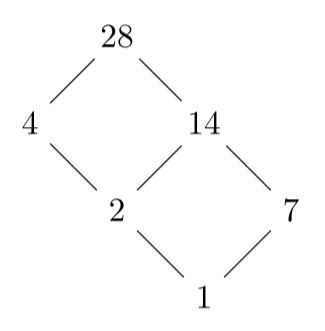
\includegraphics[scale=0.5]{hasse-diagram-1}
    \end{center}

    Die Teilmengenrelation $\subseteq$ auf der Menge $\mathcal{P}(\{a,b,c\})$, als Hasse-Diagramm dargestellt:
    \vspace{-\topsep}
    \begin{center}
        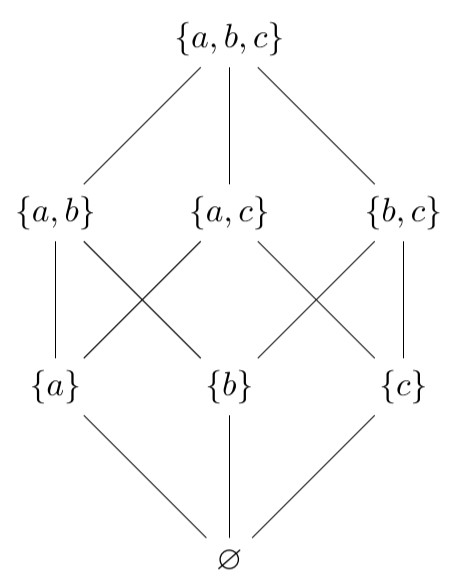
\includegraphics[scale=0.3]{hasse-diagram-2}
    \end{center}
\end{multicols}

    \section{Rekursive Strukturen und die natürlichen Zahlen}\label{sec:rekursive-strukturen-und-die-naturlichen-zahlen}

\subsection{Struktur der natürlichen Zahlen}\label{subsec:struktur-der-naturlichen-zahlen}

Wir listen einige Grundtatsachen über die Struktur der natürlichen Zahlen $\N$ auf:
\begin{itemize}
    \item Die Zahl 0 ist eine natürliche Zahl.
    \item Jede natürliche Zahl $k$ hat genau einen Nachfolger $k + 1$.
    Der Nachfolger jeder natürlichen Zahl ist wiederum eine natürliche Zahl.
    \item Die Zahl 0 ist die einzige natürliche Zahl, die kein Nachfolger ist.
    \item Natürliche Zahlen mit gleichem Nachfolger sind gleich.
    \item Enthält die Menge $X$ die 0 und mit jeder natürlichen Zahl $k$ auch deren Nachfolger $k + 1$, so bilden die natürlichen Zahlen $\N$ eine Teilmenge von $X$.
\end{itemize}
Das letzte Axiom heisst \emph{Induktionsaxiom}, da auf ihm die Beweismethode der vollständigen Induktion beruht.

\begin{definition}{}
    Die Ordnung $\leq$ auf den natürlichen Zahlen ist durch \[x \leq y \coloneqq \exists k \in \N (x + k = y)\] gegeben.
    Wir schreiben \[x < y \coloneqq x \leq \land x \neq y\]
\end{definition}

\subsection{Die vollständige Induktion}\label{subsec:die-vollstandige-induktion}

Die Induktion ist eine sehr wichtige Beweismethode in der Mathematik und in der Informatik.
Beim klassischen Induktionsbeweis geht es darum, zu zeigen, dass eine Aussage für alle natürlichen Zahlen gilt.
Sie ist folgendermassen aufgebaut:
\begin{enumerate}
    \item \textbf{Induktionsanfang:} Zeige, dass die Aussage für $n = 1$ gilt.
    \item \textbf{Induktionshypothese:} Wir nehmen an, dass die Aussage für ein allgemeines $n \in \N$ gültig ist.
    \item \textbf{Induktionsschritt:} Zeige, dass aus der Gültigkeit der Aussage für $n$ (Induktionshypothese) die Gültigkeit der Aussage für $n + 1$ folgt.
\end{enumerate}
Eine verallgemeinerte Form der Induktion erlaubt eine stärkere Induktionshypothese, nämlich dass die Aussage gültig \emph{für alle $k \leq n$} sei.

\textbf{Beispiel (Induktion):} Beweise mit der vollständigen Induktion, dass folgendes für alle $n \in \N$ gilt: \[\sum \limits_{i=0}^n 2^i = 2^{n+1} - 1\]

\textbf{Induktionsanfang (B.C.):} n = 0 \[2^0 = 1 = 2^1 - 1\]

\textbf{Induktionshypothese (I.H.):} $\forall n \in \N$ \[\sum \limits_{i=0}^n 2^i = 2^{n+1} - 1\]

\textbf{Induktionsschritt (I.S.):} $n \rightarrow n + 1$
\begin{align*}
    \sum \limits_{i=0}^{n+1} 2^i &= \sum \limits_{i=0}^{n} 2^i + 2^{n+1} \\
    &\stackrel{\text{IH}}{=} 2^{n+1} - 1 + 2^{n+1} \\
    &= 2 \cdot 2^{n+1} - 1 \\
    &= 2^{n+2} - 1
\end{align*}

% TODO: Beispiel rekursiver Algorithmus

% TODO: Beispiel rekursive Definitionen






    \section{Zahlentheorie}\label{sec:zahlentheorie}

\begin{definition}{Menge der ganzen Zahlen}
    Analog zu unserem Vorgehen mit den natürlichen Zahlen wollen wir auch die \emph{ganzen Zahlen} informell einführen.
    Wir definieren \[\Z \coloneqq \{\dots,-2,-1,0,1,2,\dots\}\]
\end{definition}

\begin{definition}{Rechenregeln auf $\Z$}
    Für alle $r,s,z \in \Z$ gelten folgende Gleichungen:
    \begin{align*}
        -1 \cdot z &= -z \\
        -(-z) &= z \\
        -z + z &= 0 & \text{Inverse Elemente bezüglich} \  +\\
        0 \cdot z &= 0 & \text{Absorbtion}\\
        1 \cdot z &= z &\text{Neutrales Element bezüglich} \ \cdot\\
        0 + z &= z &\text{Neutrales Element bezüglich} \ +\\
        r(sz) &= (rs)z &\text{Assoziativität von} \ \cdot\\
        r + (s + z) &= (r + s) + z &\text{Assoziativität von} \ +\\
        rs &= sr &\text{Kommutativität von} \ \cdot\\
        r + s &= s + r &\text{Kommutativität von} \ +\\
        r(s + z) &= rs + rz &\text{Distributivität}\\
        rx = ry &\Rightarrow x = y \lor r = 0 &\text{Kürzbarkeit}
    \end{align*}
\end{definition}

\begin{definition}{Definitionen}
    Wir definieren die \emph{Substraktion} $-\ : \Z \times \Z \rightarrow \Z$ durch \[x - y \coloneqq x + (-y)\text{,}\]
    die \emph{Betragsfunktion} $| \cdot | : \Z \rightarrow \N$ durch \[ |z| =
    \begin{cases}
        z$ falls $z \in \N \\ -1 \cdot z$ sonst$
    \end{cases}\]
    und die Relation $\leq$ durch \[x \leq y \coloneqq \exists n \in \N \left(x + n = y\right)\text{.}\]
\end{definition}

\subsection{Teilbarkeit und der Euklidische Algorithmus}\label{subsec:teilbarkeit-und-der-euklidische-algorithmus}

\begin{definition}{Definition}
    Sind $x,y \in \Z$ ganze Zahlen, so sagen wir, dass \emph{x ein Teiler von y} ist, falls es ein $k \in \Z$ gibt mit $xk = y$.
    Wir schreiben in diesem Fall $x | y$.
    Es gilt also \[x | y \coloneqq \exists k \in Z \left( y = xk \right)\]
    Mit $T(y)$ bezeichnen wir die Menge aller natürlichen Zahlen, welche Teiler von $y$ sind, also $T(x) = \{ x \in \N \mid x | y \}$.
\end{definition}

\textbf{Bemerkung:} Die Teilbarkeitsrelation ist reflexiv und transitiv auf der Menge $\Z$, auf der Menge $\N$ ist die Teilbarkeitsrelation sogar eine Halbordnung.

\begin{definition}{Satz}
    Sind $n,m \in \N \backslash \{0\}$, dann gibt es eindeutig bestimmte Zahlen $k,r \in \N$, sodass Folgendes gilt:
    \begin{multicols}{2}
        \begin{itemize}
            \item $m = kn + r$
            \item $r < n$
        \end{itemize}
    \end{multicols}
    Wir sagen in diesem Zusammenhang, dass die Zahl $r$ der Rest von der ganzzahligen Division von $m$ durch $n$ ist.
\end{definition}

\begin{definition}{KgV und ggT}
    Seien $n,m \in Z$.
    Wir definieren das \emph{kleinste gemeinsame Vielfache von $n$ und $m$} als \[kgV(n,m) \coloneqq \min \{ k \in N \mid n|k \land m|k \}.\]
    Ist $n \neq 0$ oder $m \neq 0$, dann definieren wir den \emph{grössten gemeinsamen Teiler von $n$ und $m$} als \[ggT(n,m) \coloneqq \max \{ k \in \N \mid k|n \land k|m \}.\]
\end{definition}

\begin{definition}{Satz (Euklidischer Algorithmus)}
    Für $n,m \in \N$ mit $0 < n < m$ gilt \[ggT(n,m) = ggT(n,m-n) = ggT(m,m-n).\]
\end{definition}

\begin{mainbox}{Rezept: Euklidischer Algorithmus}
    \begin{enumerate}
        \item Grössere durch kleinere Zahl dividieren.
        \item Divisor durch Rest dividieren.
        Diesen Schritt so oft wiederholen, bis kein Rest übrig bleibt.
        \item Ergebnis aufschreiben.
    \end{enumerate}
\end{mainbox}

\textbf{Beispiel: $ggT(442, 255)$}
\vspace{-\topsep}
\begin{enumerate}
    \item $442 : 255 = 1$ Rest $187$
    \item $255 : 187 = 1$ Rest $68 \\
    187 : 68 = 2$ Rest $51 \\
    68 : 51 = 1$ Rest $17 \\
    51 : 17 = 3$ Rest $0$
    \item $ggT(442, 255) = 17$
\end{enumerate}

\begin{subbox}{}
    Zwei ganze Zahlen $x,y$ heissen \emph{teilerfremd}, wenn $ggT(x,y) = 1$ gilt.
\end{subbox}

\begin{definition}{Lemma von Bézout}
    Sind $x,y \in \Z$ mit $x,y \neq 0$, dann gibt es ganze Zahlen $a,b$, sodass \[ggT(x,y) = ax + by\] gilt.
    Die Zahlen $a$ und $b$ werden \emph{Bézout-Koeffizienten} genannt.
\end{definition}

\textbf{Beispiel:} Berechnen Sie $ggT(135, 480)$ und gleichzeitig die $x,y$ mit $ggT(135, 480) = 135x + 480y$.
Wir wenden den sogenannten \emph{erweiterten Euklidischen Algorithmus} an:
\begin{alignat*}{2}
    480 &= 3 \cdot 135 + 75 \quad \quad &&\Leftrightarrow 75 = 480 - 3 \cdot 135 \\
    135 &= 1 \cdot 75 + 60 &&\Leftrightarrow 60 = 135 - 1 \cdot 75 = 135 - (480 - 3 \cdot 135) = -480 + 4 \cdot 135 \\
    75 &= 1 \cdot 60 + 15 &&\Leftrightarrow 15 = 75 - 1 \cdot 60 = 480 - 3 \cdot 135 - (-480 + 4 \cdot 135) = 2 \cdot 480 - 7 \cdot 135 \\
    60 &= 4 \cdot 15 + 0
\end{alignat*}
Wir erhalten also $ggT(480, 135) = 15 = -7 \cdot 135 + 2 \cdot 480$, also $x = -7$ und $y = 2$.

\subsection{Primzahlen}\label{subsec:primzahlen}

\begin{definition}{Definition}
    Eine natürliche Zahl $p$ ist eine \emph{Primzahl}, wenn $|T(p)| = 2$ gilt.
    Die Menge der Primzahlen bezeichnen wir mit $\P$.
\end{definition}

\textbf{Bemerkung:} Ist $p$ eine Primzahl, dann gilt $T(p) = \{ 1,p \}$.

\begin{definition}{Lemma von Euklid}
    Für $p \in \N$ mit $p \neq 1$ gilt: \[\forall n,m \in \N \left( p|nm \Rightarrow p|n \lor p|m \right) \Leftrightarrow p \in \P.\]
    Mit anderen Worten: Primzahlen haben die Eigenschaft, dass sie mit jedem Produkt auch mindestens einen der Faktoren teilen.
    Umgekehrt ist auch jede von 1 verschiedene natürliche Zahl mit dieser Eigenschaft eine Primzahl.
\end{definition}

\begin{definition}{}
    Jede ganze Zahl $z$ mit $z \notin \{ -1,1 \}$ besitzt einen Primfaktor (einen Teiler, der eine Primzahl ist).
    Formal können wir dies als \[\forall z \in \Z \left( z \notin \{-1,1 \} \Rightarrow T(z) \cap \P \neq 0 \right)\] ausdrücken.
\end{definition}

\begin{definition}{Theorem}
    Jede natürliche Zahl grösser als 1 ist das Produkt von endlich vielen Primzahlen.
\end{definition}

\begin{definition}{Primfaktorzerlegung}
    Es sei $p_i$ jeweils die $i$-te Primzahl.
    Für jede natürliche Zahl $n > 1$ gibt es eine eindeutig bestimmte, endliche Folge $a_1,\cdots,a_k$ von natürlichen Zahlen mit $a_k \neq 0$, sodass \[n = \prod_{i=1}^k p_i^{a_i}\] gilt.
\end{definition}

\subsection{Modulare Arithmetik}\label{subsec:modulare-arithmetik}

In der modularen Arithmetik geht es darum mit Restklassen zu rechnen.
Die Grundlage der modularen Arithmetik ist die ``kongruent modulo''-Relation.

\begin{definition}{Definition}
    Es sei $n \in \N$ beliebig.
    Wir definieren eine Relation $\equiv_n$ auf $\Z$ wie folgt: \[r \equiv_n s \coloneqq n|(r-s).\]
    Gilt für $r,s \in \Z$ die Relation $r \equiv_n s$, dann sagen wir, dass $r$ gleich $s$ modulo $n$ ist und wir schreiben \emph{r = s mod n}.
\end{definition}

\textbf{Bemerkung:} Die Relation $\equiv_n$ ist für jede natürliche Zahl $n$ eine Äquivalenzrelation auf $\Z$.

\textbf{Bemerkung:} Es sei $n \in \N$ beliebig.
Für je zwei ganze Zahlen $x$ und $y$ gilt $x \equiv_n y$ genau dann, wenn $x$ und $y$ denselben Rest bei Division durch $n$ haben.

\textbf{Folgerung:} Es sei $n \in \N$ beliebig.
Jede ganze Zahl $z$ steht mit genau einer natürlichen Zahl aus $\{0,\cdots,n-1\}$ in der Relation $\equiv_n$.

\begin{definition}{Definition}
    Es sei $n \in \N$ beliebig.
    Für jede ganze Zahl $z$ bezeichnen wir mit \[[z]_n \coloneqq \{ x \in \Z \mid x \equiv_n z \}\] die Äquivalenzklasse von $z$ bezüglich der Relation $\equiv_n$ und nennen diese auch die \emph{Restklassen} von $z$.
    Abkürzend bezeichnen wir $[z]_n$ auch mit $\overline{k}$, wenn $k \in \{ 0, \cdots, n-1\}$ und $z \equiv_n k$ gilt.
\end{definition}

\textbf{Folgerung:} Es sei $n \in \N$ beliebig.
Es gilt \[[z]_n = \{ z + yn \mid y \in \Z \} = \{\cdots, z-3n, z-2n, z-n,z,z+n, z+2n, z+3n, \cdots \}.\] Damit wir mit Restklassen sinnvoll rechnen können, müssen wir uns davon überzeugen, dass die Rechenoperationen unabhängig von der Wahl von Repräsentanten sind.

\textbf{Bemerkung:} Es sei $n \in \N$ beliebig.
Für ganze Zahlen $x, x'$ und $y, y'$ gelten:
\vspace{-\topsep}
\begin{itemize}
    \item $[x] = [x'] \land [y] = [y'] \Rightarrow [x + y] = [x' + y']$
    \item $[x] = [x'] \land [y] = [y'] \Rightarrow [xy] = [x'y']$
\end{itemize}

\begin{definition}{Definition}
    Es sei $n \in \N$ beliebig.
    Die Menge aller Restklassen von $\Z$ modulo $n$ bezeichnen wir mit \[\Z/n = \{ [z]_n \mid z \in \Z \} = \{ \overline{k} \mid 0 \leq k < n - 1 \land z \equiv_n k \} = \{\overline{0}, \overline{1}, \overline{2}, \cdots, \overline{n-1} \}.\]
    Wir definieren zwei Verknüpfungen $\cdot : (\Z/n)^2 \rightarrow \Z/n$ und $+ : (\Z/n)^2 \rightarrow \Z/n$ durch die Zuordnungen \[[x]_n + [y]_n \coloneqq [x + y]_n\] und \[[x]_n \cdot [y]_n \coloneqq [xy]_n.\]
\end{definition}

% TODO: Bemerkungen

\subsubsection{Chinesischer Restsatz}

\begin{definition}{Chinesischer Restsatz}
    Es seien $n_1,\dots,n_k \in \N_{>1}$ paarweise teilerfremd und weiter $y_1,\dots,y_k \in \Z$ beliebig.
    Es gibt genau eine natürliche Zahl $x < \prod_{i=1}^k n_i$ so, dass die Lösungsmenge des Systems
    \begin{align*}
        &x \equiv_{n_1} y_1 \\
        &x \equiv_{n_2} y_2 \\
        &\vdots \\
        &x \equiv_{n_k} y_k
    \end{align*}
    der Menge $[x]_{\prod_{i=1}^k} n_i$ entspricht.
\end{definition}

\textbf{Bemerkung:} Aus dem chinesischen Restsatz folgt, dass wir, um ein System simultaner Kongruenzen zu lösen, bloss eine Lösung davon kennen müssen.
Durch sukzessive Substitution genügt es also jeweils eine Lösung von einem System mit zwei Gleichungen zu finden, um beliebige Systeme lösen zu können.

\begin{subbox}{Algorithmus}
    Wir wollen ein System simultaner Kongruenzen mit zwei Gleichungen lösen, etwa
    \begin{align*}
        &x \equiv_{n_1} y_1 \\
        &x \equiv_{n_2} y_2
    \end{align*}
    mit $n_1$ und $n_2$ teilerfremd.
    Wir gehen schrittweise wie folgt vor:
    \begin{enumerate}
        \item Durch sukzessives Teilen mit Rest erhalten wir ganze Zahlen $a,b$ mit $an_1 + bn_2 = 1$.
        \item Wir setzen $x \coloneqq y_1 bn_2 + y_2 an_1$.
    \end{enumerate}
\end{subbox}

\begin{definition}{Lemma}
    Ist $a \in \Z/n$ mit $n > 0$ invertierbar, dann ist die Funktion
    \begin{align*}
        &f : \Z/p \rightarrow \Z/p \\
        &f(x) = \overline{a} \cdot x
    \end{align*}
    surjektiv.
\end{definition}

\begin{definition}{Kleiner fermatscher Satz}
    Ist $p \in \P$ und $a$ kein Vielfaches von $p$, dann gilt \[a^{p-1} \equiv_p 1.\]
\end{definition}

\textbf{Beispiel (Chinesischer Restsatz):}
\begin{align*}
    x &\equiv_{73} 5 \\
    x &\equiv_{3} 1 \\
    x &\equiv_{11} 6
\end{align*}

Wir setzen $n_1 = 73$, $n_2 = 3$ und $n_3 = 11$, und rechnen das Produkt davon aus: $n = n_1 \cdot n_2 \cdot n_3 = 2409$.

Anschliessend rechnen wir $N_1 = n_2 \cdot n_3 = 33$, $N_2 = n_1 \cdot n_3 = 803$ und $N_3 = n_1 \cdot n_2 = 219$ aus.
\begin{align*}
[33]
    _{73}^{-1} &\stackrel{*}{=} [31]_{73} \\
    [803]_3^{-1} &= [2]_3^{-1} = [2]_3 \quad \longrightarrow \quad [2]_3 \cdot [2]_3 = [4]_3 = [1]_3 \\
    [219]_{11}^{-1} &= [10]_{11}^{-1} = [10]_{11} \quad \longrightarrow \quad [10]_{11} \cdot [10]_{11} = [100]_{11} = [1]_{11}
\end{align*}
Wir haben also \[x = 5 \cdot 33 \cdot 31 + 1 \cdot 803 \cdot 2 + 6 \cdot 219 \cdot 10 = 19861\] und damit \[[19861]_{2409} = [589]_{2409}.\]

Die gesamte Lösungsmenge lautet $\{ 589 + k \cdot 2409 : k \in \Z \}.$

\begin{alignat*}{2}
    \text{(*)}\quad &73 = 2 \cdot 33 + 7 \quad \quad &&\Rightarrow 7 = 73 - 2 \cdot 33 \\
    &33 = 4 \cdot 7 + 5 &&\Rightarrow 5 = 33 - 4 \cdot 7 = 33 - 4 \cdot (73 - 2 \cdot 33) = 9 \cdot 33 - 4 \cdot 73 \\
    &7 = 1 \cdot 5 + 2 &&\Rightarrow 2 = 7 - 5 = 73 - 2 \cdot 33 - (9 \cdot 33 - 4 \cdot 73) = 5 \cdot 73 - 11 \cdot 33 \\
    &5 = 2 \cdot 2 + 1 &&\Rightarrow 1 = 5 - 2 \cdot 2 = 9 \cdot 33 - 4 \cdot 73 - 2 \cdot (5 \cdot 73 - 11 \cdot 33) = 31 \cdot 33 - 14 \cdot 73
\end{alignat*}

\textbf{Beispiel (Multiplikative Inverse):} Welche Elemente von $\Z/12$ besitzen multiplikative Inverse?
\begin{align*}
    ggT(12,1) = 1 &\Rightarrow [1]_{12}^{-1} = [1]_{12} \\
    ggT(12,5) = 1 &\Rightarrow [5]_{12}^{-1} = [5]_{12} \\
    ggT(12,7) = 1 &\Rightarrow [7]_{12}^{-1} = [7]_{12} \\
    ggT(12,11) = 1 &\Rightarrow [11]_{12}^{-1} = [11]_{12}
\end{align*}

\textbf{Beispiel (Verknüpfungstabelle):} Skizzieren Sie die Verknüpfungstabelle von $\Z/4$ und markieren Sie die Elemente, die kein multiplikatives Inverses besitzen.

\begin{center}
    \begin{tabular}{c|cccc}
        $\cdot$ & $0$ & $1$ & $2$ & $3$ \\
        \hline
        0       & 0   & 0   & 0   & 0   \\
        1       & 0   & 1   & 2   & 3   \\
        2       & 0   & 2   & 0   & 2   \\
        3       & 0   & 3   & 2   & 1
    \end{tabular}
\end{center}

\textbf{Beispiel (Multiplikatives Inverse):} Bestimmen Sie das multiplikative Inverse von $\overline{6111}$ in $\Z/6211$.

Wir wenden den erweiterten euklidischen Algorithmus an:
\begin{alignat*}{2}
    &6211 = 1 \cdot 6111 + 100 \quad \quad &&\Leftrightarrow 100 = 6211 - 6111 \\
    &6111 = 61 \cdot 100 + 11 &&\Leftrightarrow 11 = 6111 - 61 \cdot 100 = 6111 - 61 \cdot (6211 - 6111) = 62 \cdot 6111 - 61 \cdot 6211 \\
    &100 = 9 \cdot 11 + 1 &&\Leftrightarrow 1 = 100 - 9 \cdot 11 = 6211 - 6111 - 9 \cdot (62 \cdot 6111 - 61 \cdot 6211) = 550 \cdot 6211 - 559 \cdot 6111
\end{alignat*}

Damit haben wir: \[[6111]_{6211}^{-1} = [-559]_{6211} = [5652]_{6211}\]

\textbf{Beispiel (Chinesischer Restsatz):}
\begin{align*}
    x &\equiv_{7} 5 \\
    x &\equiv_{3} 2 \\
    x &\equiv_{8} 1
\end{align*}
Zuerst überprüfen wir, dass alle Moduli teilerfremd sind (Voraussetzung für den chinesischen Restsatz): \[ggT(3,7) = ggT(3,8) = ggT(7,8) = 1\]
Dann berechnen wir: $n = 3 \cdot 7 \cdot 8 = 168$ und $N_1 = n_2 \cdot n_3 = 7 \cdot 8 = 56$, $N_2 = n_1 \cdot n_3 = 3 \cdot 8 = 24$, $N_3 = n_1 \cdot n_2 = 3 \cdot 7 = 21$
\begin{align*}
    &[N_1]_{n_1}^{-1} = [56]_3^{-1} = [2]_3^{-1} = [2]_3 \\
    &[N_2]_{n_2}^{-1} = [24]_7^{-1} = [3]_7^{-1} = [5]_7 \\
    &[N_3]_{n_3}^{-1} = [21]_8^{-1} = [5]_8^{-1} = [5]_8
\end{align*}
Damit ist \[x = 2 \cdot 56 \cdot 2 + 5 \cdot 24 \cdot 5 + 1 \cdot 21 \cdot 5 = 929\] und wir schliessen ab mit \[[929]_{168} = [89]_{168}.\]
Die Lösungsmenge lautet: $\{89 + k \cdot 168 : k \in \Z\}$
\end{document}